
\section{Amplitude modulation}

We want to solve equation \ref{eq:to_solve} when a amplitude modulated external force is applied, this force follows from equation \ref{eq:force_q3}.\\

\begin{equation}
    m \ddot{x}(t)+m\frac{\omega}{Q}\dot{x}(t)+m \omega^2 x(t) = F(t)
    \label{eq:to_solve}
\end{equation}

\begin{equation}
    F(t) = F_0 t\frac{T-t}{T^2}= F_0 \frac{t}{T} - F_0 \frac{t^2}{T^2}
    \label{eq:force_q3}
\end{equation}

To solve equation \ref{eq:to_solve} numerically we first have to split the second order differential equations into a system of two first order equations. We do this by substituting two new time dependant functions for $y$, namely $u(t)$ and $v(t)$ equal to $y(t)$ and $y'(t)$ respectively. We can then derive the following system:\\

\begin{equation*}
    \left\{ \begin{matrix} \mbox{u(t) = y(t)}\\
    \mbox{v(t) = y'(t)} \end{matrix} \right.
\end{equation*}

So that their derivatives become:\\

\begin{equation*}
    \left\{ \begin{matrix} \mbox{u'(t) = y'(t) = v(t)}\\
    \mbox{v'(t) = y"(t)} \end{matrix} \right.
\end{equation*}

If we then substitute in these equations into the second order differential equation we get the following system:\\

\begin{align*}
    u'(t) &= y'(t) = v(t)\\
    v'(t) &= y''(t)\\
    F(t) &= m y''(t)+m\frac{\omega}{Q}y'(t)+m \omega^2 y(t)\\
\end{align*}

\begin{align*}
    v'(t) &= y''(t) = 1/m \cdot F(t) - \omega/Q\cdot y'(t)-\omega^2\cdot y(t)\\
    v'(t) &= 1/m\cdot F(t) - \omega/Q\cdot v(t)-\omega^2\cdot u(t)
\end{align*}

So that we now have the following system of of first-order linear differential equations:\\

\begin{align}
    v'(t) &= 1/m\cdot F(t)-\omega/Q\cdot v(t)- \omega^2\cdot u(t)\\
    u'(t) &= v(t)
\end{align}

This system can be easily solved numerically using the python code shown in the appendix section \ref{PythonCode}. We can then use a similar program to plot the nine different scenarios, these are shown in figure \ref{fig:fig_Q3}.\\
\newpage

\begin{figure}[!h]
    \centering
    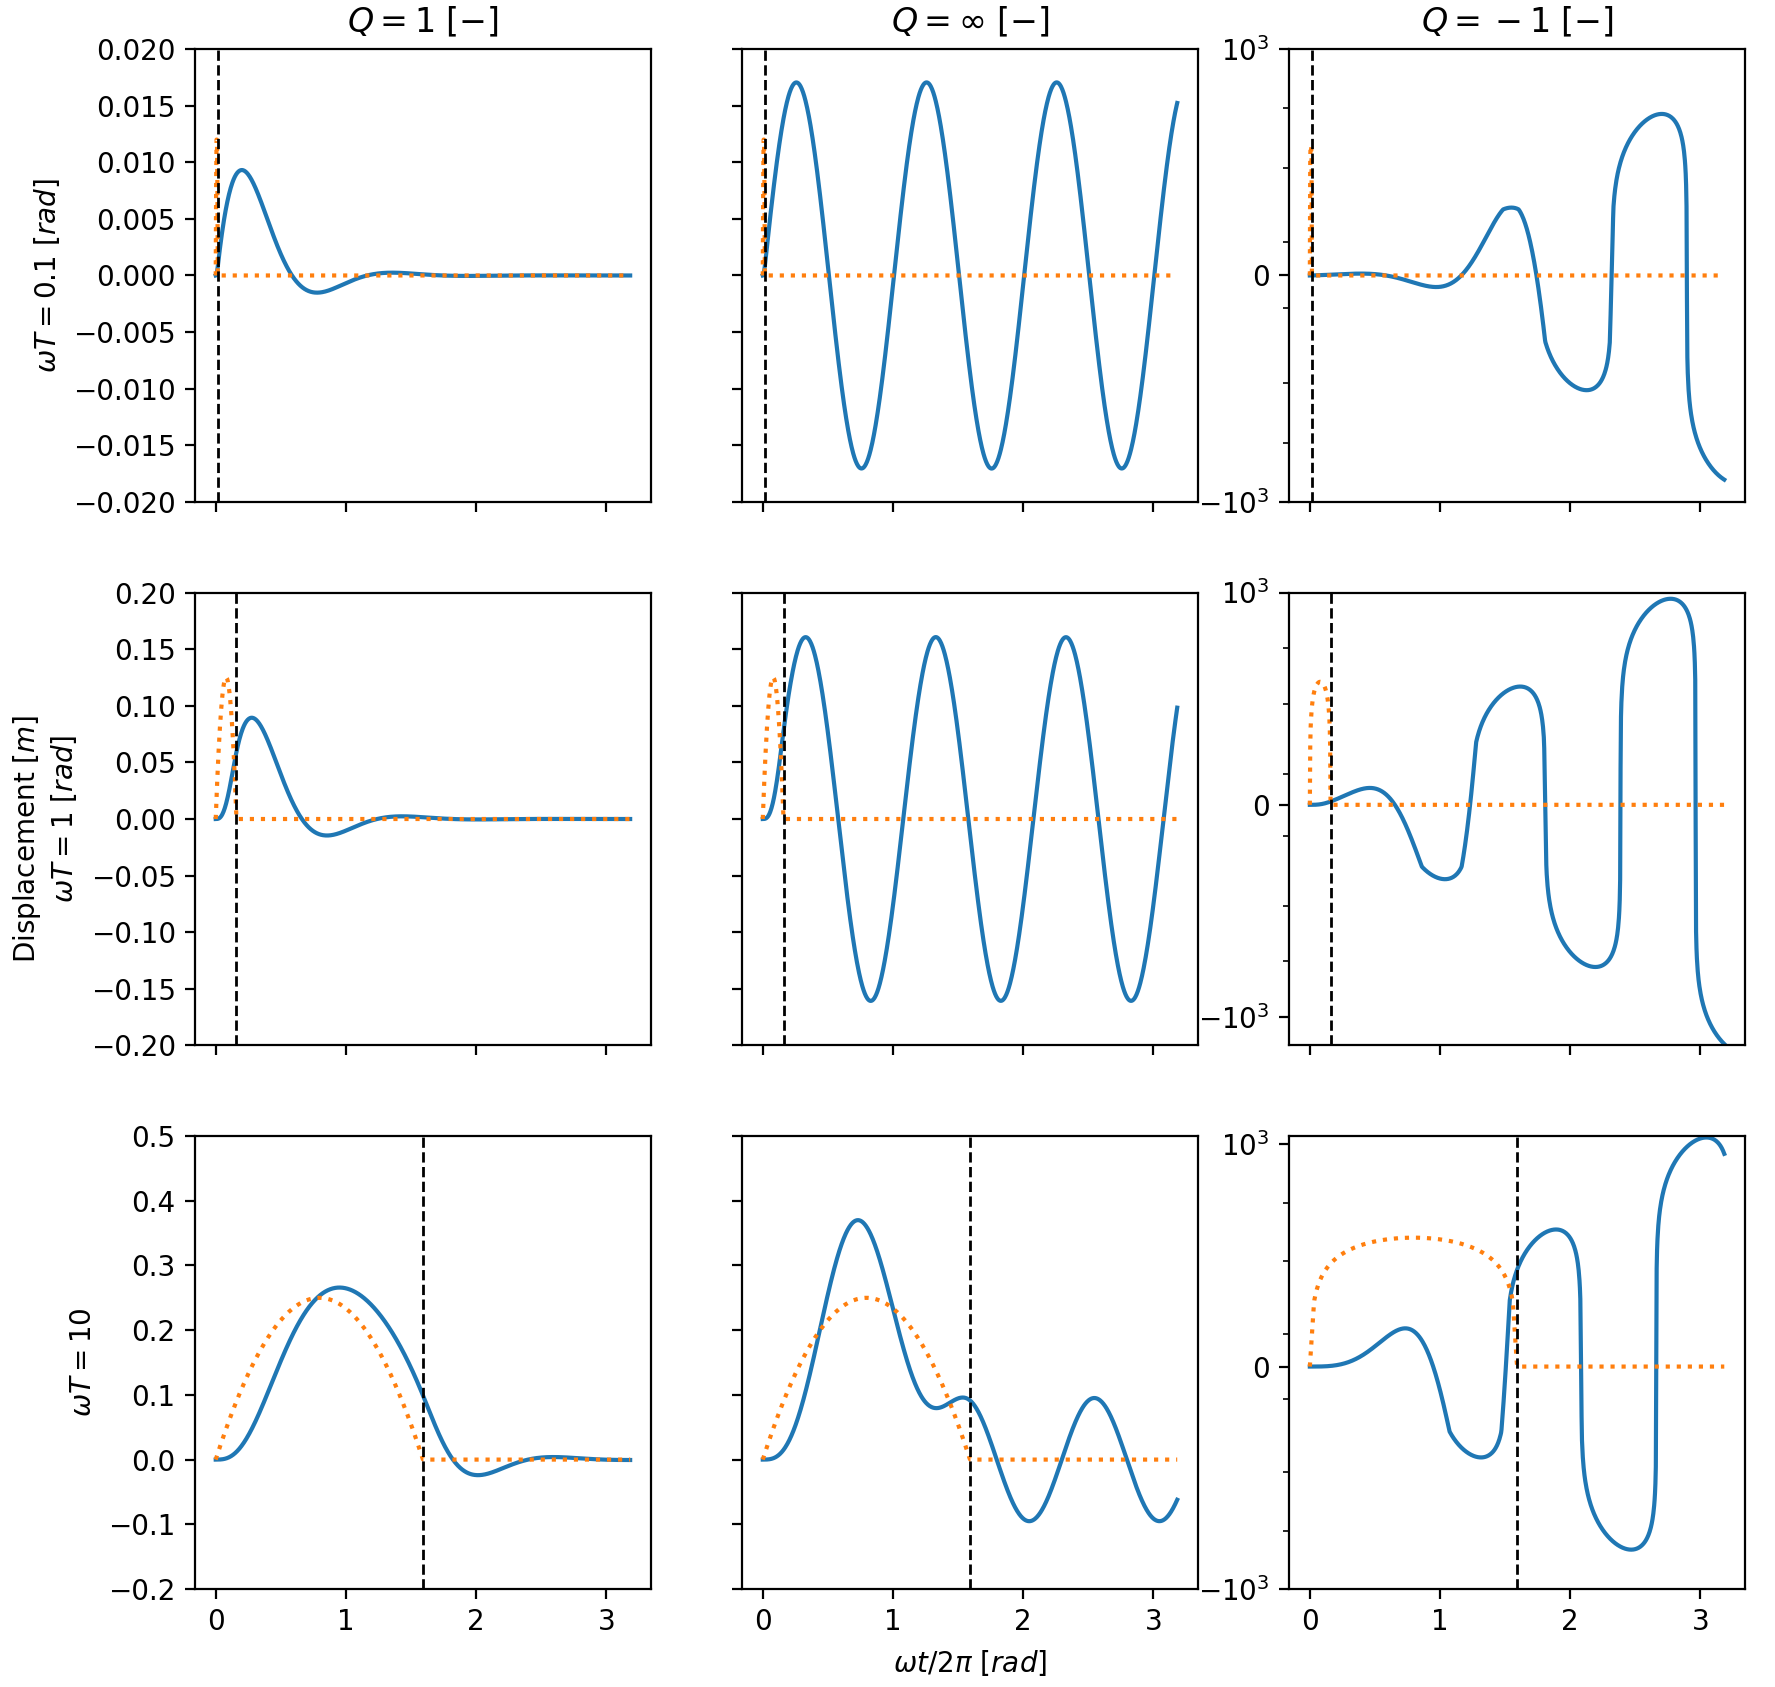
\includegraphics[width=.7\linewidth,keepaspectratio]{figures/Q3_omega_q_plot.png}
    \caption{The resulting oscillations for a parabolic force modulation. Here the displacement of the mass is plotted as a solid line and the force is plotted as the dashed line. The force is the same in all graphs but is scaled to emphasise the form. }
    \label{fig:fig_Q3}
\end{figure}

When looking at the graph we can see the different values of $\omega T$ plotted in rows and the different values of $Q$ in columns, all plots share the same time domain but only plots on the same row and in the first and second column share displacement axis.\\
The different values of $\omega T$ make noticeable differences in the graphs, the smallest value $\omega T = 0.1$ acts a lot like an impulse function, applying a short but strong force to set de oscillator into motion. We can see that for different quality factors the system reacts differently, for a normal friction force the system gradually returns to the equilibrium position, for $Q = \infty$ there is no friction force and the system start oscillating forever and looks like it had a starting velocity due to the short impulse force, for the quality factor of $Q = -1$ the friction force actually puts more energy into the system causing it to spiral out of control.
For the higher values of $\omega T$ we can see that the force is no longer representative of an impulse, meaning that the acceleration is not instantaneous, in the graph this can be seen by the small curve at the start of the plots where the oscillating mass needs to gain energy first. The different quality factors have the same effect as before.
The other noticeable effect is that in the bottom middle graph for $Q=\infty$ and $\omega T = 10$ we can see that the duration of the force applied is to long, at about 7 seconds the force starts to work against the oscillation thus having the adverse to the intended effect of a driving force. This effect can also be seen though less noticeably so with the graph to the left where the force is also pushing the mass away from equilibrium while the mass is already moving towards the equilibrium position.
It is clear from the plots that for this type of modulation the ringdown is shorter than the previous modulation methods thus it is easier to transfer more signals using this method.\\